\section{Results}
\label{sec:results}

\subsection{RQ-A: Honest agent vs.\ baselines}
\label{sec:results-baselines}

\begin{table}[t]
\caption{Leak-free agent vs.\ non-LLM baselines (top-1 service; both = service and
fault type correct).}
\label{tab:baselines}
\begin{tabular}{lccl}
\toprule
Method & Service & Both & Degradation behavior \\
\midrule
Statistical rule tree & ${\sim}48\%$ & 38\% & flat; kernel-blind \\
RCAEval/mmbaro & 46\% (AC@3 63\%) & --- & flat, 100$\to$5\% traces \\
MicroRank / TraceRCA & ${\sim}0\%$ / ${\sim}5\%$ & --- & floor, no cliff \\
\textbf{Agent (leak-free)} & \textbf{83--87\%} & \textbf{57\%} & \S\ref{sec:results-trace} \\
\bottomrule
\end{tabular}
\end{table}

The leak-free agent roughly doubles both baselines on localization
(Table~\ref{tab:baselines}) at ${\sim}25$k input tokens (50--73\% served from prompt
cache) and ${\sim}\$0.01$ per incident. Naive kernel-feature fusion into mmbaro changes
nothing (kernel columns rank ${\sim}195$th among its change points), and the two
non-LLM baselines fail on \emph{different} faults --- both observations motivate an
agent that reasons across modalities rather than a wider feature table.

\subsection{RQ-B: The price of leakage}
\label{sec:results-leak}

\begin{table}[t]
\caption{The honesty arc: identical incidents, progressively honest evaluation.}
\label{tab:leak}
\begin{tabular}{lccc}
\toprule
Configuration & Service & Fault & Both \\
\midrule
Leaky (run IDs, fault-named containers visible) & 74\% & 74\% & 61\% \\
Masked, original tools & 48\% & 17\% & 9\% \\
Masked, fragmented aliases (identity broken) & 26\% & 17\% & 4\% \\
Masked, generic tooling rebuilt & \textbf{83\%} & 48\% & 48\% \\
\quad + deterministic context brief (config of record) & \textbf{87\%} & \textbf{61\%} & \textbf{57\%} \\
\bottomrule
\end{tabular}
\end{table}

Naming hints alone were worth ${\sim}26$ points of localization and ${\sim}57$ points
of fault classification --- fault labels were effectively read off the run identifier.
The fragmented-alias row isolates the identity-preservation requirement of
\S\ref{sec:leakage}. Honest tooling then \emph{exceeded} the leaky localization number
(Fig.~\ref{fig:honesty}).

\begin{figure}[t]
\centering
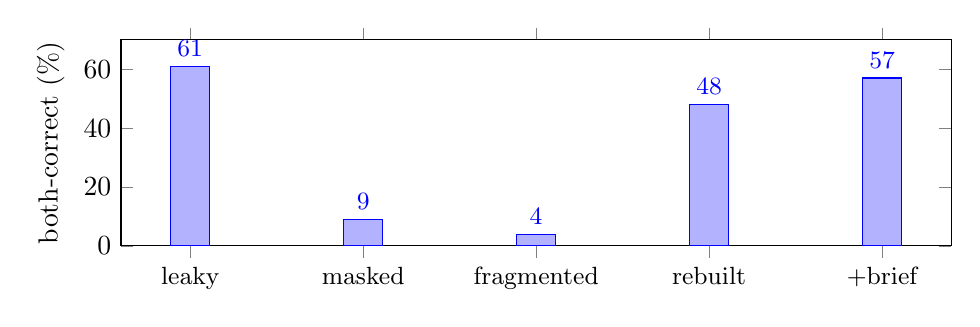
\begin{tikzpicture}
\begin{axis}[width=\columnwidth, height=4.2cm, ybar, bar width=14pt,
  ylabel={both-correct (\%)}, ymin=0, ymax=70, ytick={0,20,40,60},
  symbolic x coords={leaky, masked, fragmented, rebuilt, +brief},
  xtick=data, x tick label style={font=\small}, nodes near coords,
  every node near coord/.append style={font=\small}]
\addplot coordinates {(leaky,61) (masked,9) (fragmented,4) (rebuilt,48) (+brief,57)};
\end{axis}
\end{tikzpicture}
\caption{The honesty arc (both-correct on identical incidents): removing leaks
collapses performance; rebuilding generic evidence recovers --- and on localization
exceeds --- it.}
\label{fig:honesty}
\end{figure}

\subsection{RQ-C: What is kernel telemetry worth?}
\label{sec:results-kernel}

\begin{table}[t]
\caption{Kernel-tier ablation (23 incidents $\times$ 4 tiers; brief on, skills off).}
\label{tab:kernel}
\begin{tabular}{lcccc}
\toprule
Kernel view & Service & Fault & Both & Agent calls \\
\midrule
L1+L2+L3 & 83\% & 61\% & 61\% & \textbf{9.1} \\
L1 only & 74\% & 48\% & \textbf{43\%} & 10.1 \\
L3 only & 78\% & 57\% & 57\% & 10.0 \\
none & 78\% & 57\% & 57\% & 12.2 \\
\bottomrule
\end{tabular}
\end{table}

\textbf{K1.} Removing kernel telemetry entirely costs $\le$4 points (within the noise
band) but $+34\%$ investigation effort: with strong cross-modality tooling, kernel's
robust value at full telemetry is \emph{efficiency}, not rescue. \textbf{K2.} The one
stable loss is induced-DB-latency \emph{typing}: wait attribution converts ``the
datastore is the locus'' into ``induced latency, not an application bug''.
\textbf{K3.} \emph{A partial kernel view is worse than none}: raw KPIs without
interpretive framing send the agent chasing kernel noise ($-14$ points vs.\
kernel-blind; four families lost, none gained) --- representation quality dominates
kernel presence. \textbf{K4.} The pre-registered hypothesis that removing kernel
causes the largest drop on blind-spot faults is \emph{not confirmed at full
telemetry}: kernel-decisive families hold 85\% service in every tier because our
limit-signal/topology/host tools absorbed the signal (recorded in the
pre-registration amendment log). The interaction test sharpens this
(\S\ref{sec:results-interact}): the kernel advantage does not grow under trace
\emph{thinning} either --- but kernel \emph{does} compensate under complete trace
\emph{removal}, restoring both locus and typing on induced DB latency. H2 is thereby
refined rather than merely refuted: kernel is a compensating channel under modality
loss, not under modality thinning. Behaviorally, the kernel-blind agent wastes
${\sim}30\%$ of calls re-probing the empty modality unless the tool answers
definitively once --- an agent-design lesson in its own right.

\subsection{RQ-D: Telemetry degradation --- no cliff on any axis}
\label{sec:results-trace}

\begin{table}[t]
\caption{Degradation axes on the agent (23 incidents per condition; both-correct;
single-run noise band ${\pm}9$ points). Full per-condition tables in the artifact.}
\label{tab:degradation}
\begin{tabular}{llll}
\toprule
Axis & Range tested & Both-correct span & Verdict \\
\midrule
Traces & 100\%$\to$5\% retention & 43--57\% & flat (10\% scores best) \\
Metrics & 5\,s$\to$60\,s scrape & 43--52\% & flat (30\,s scores best) \\
Logs & ALL$\to$ERROR-only & 43--57\% & flat (ERROR beats WARN) \\
Kernel & full ladder$\to$none & 43--61\% & $-4$ pts, $+34\%$ calls; L1-only worst \\
\bottomrule
\end{tabular}
\end{table}

\paragraph{Traces.} Across 100/50/25/10/5\% whole-trace retention (115 diagnoses),
both-correct stays within 43--57\% (the noise band; 10\% retention scores best), 18/23
incidents produce identical outcomes at every level, and the tool mix is constant.
Mechanism: the agent consumes spans as \emph{aggregates} --- brief latency tops and
topology edge percentiles --- which survive uniform sampling; direct raw-trace reads
are nearly absent. The baselines were flat because they never extracted trace value;
the agent is flat because its trace use is statistical and redundantly backed --- the
same curve for the opposite reason. \emph{Implication: ${\sim}20\times$ trace
collection-cost reduction without diagnostic loss} at otherwise-full telemetry.

\paragraph{Metrics.} Coarsening scrape resolution 5$\to$60\,s (92 diagnoses) moves
both-correct 43/48/52/48\% --- non-monotonic, with 30\,s scoring best, and per-family
flips balanced in both directions (pure churn). The tools compute window-level rates
and means over 60--120\,s windows; a counter needs only two samples per window, so
even 60\,s scrape preserves every delta the agent reads.

\paragraph{Logs.} Filtering ALL$\to$WARN$\to$ERROR-only (69 diagnoses) gives
57/43/52\% --- ERROR-only \emph{beats} WARN, confirming non-signal: the log tool keys
on error-class signature \emph{changes}, which survive the harshest filter by
construction. The one incident recurring in loss lists across both axes (Sock~Shop
memory-cap) is also in the A/A flip-prone set, so we make no per-family claim.

\begin{figure}[t]
\centering
\begin{tikzpicture}
\begin{axis}[width=\columnwidth, height=4.6cm,
  xlabel={degradation severity (normalized: 0 = full telemetry)},
  ylabel={both-correct (\%)}, ymin=0, ymax=70, ytick={0,20,40,60},
  xmin=-0.03, xmax=1.03, legend style={font=\scriptsize, at={(0.02,0.02)},
  anchor=south west, legend columns=2}, grid=major, grid style={dashed,gray!25}]
% noise band around the full-telemetry reference (57 +/- 9)
\addplot[draw=none, fill=gray!15, forget plot] coordinates
  {(-0.03,48) (1.03,48) (1.03,66) (-0.03,66)} \closedcycle;
\addplot+[mark=*] coordinates {(0,52) (0.25,52) (0.5,43) (0.75,57) (1,43)};
\addlegendentry{traces 100$\to$5\%}
\addplot+[mark=square*] coordinates {(0,43) (0.33,48) (0.67,52) (1,48)};
\addlegendentry{metrics 5$\to$60\,s}
\addplot+[mark=triangle*] coordinates {(0,57) (0.5,43) (1,52)};
\addlegendentry{logs ALL$\to$ERROR}
\addplot+[mark=diamond*] coordinates {(0,61) (0.33,43) (0.67,57) (1,57)};
\addlegendentry{kernel full$\to$none}
\end{axis}
\end{tikzpicture}
\caption{Both-correct under per-axis degradation (23 incidents per point; shaded band
= single-run noise around the full-telemetry reference). No axis exhibits a cliff;
the kernel dip at severity 0.33 is the L1-only tier (partial view worse than none).}
\label{fig:degradation}
\end{figure}

\paragraph{Consolidated RQ-D answer.} There is no degradation cliff at standard
operational ranges (Table~\ref{tab:degradation}, Fig.~\ref{fig:degradation}). The pre-registered cliff expectation
resolves as a \emph{robustness} result with one structural cause: the agent consumes
every modality at the aggregate level, with evidence redundant across modalities ---
when one channel thins, the fault signature usually survives in another. The one real
hazard is qualitative, not quantitative: a \emph{badly represented} modality (raw
kernel KPIs alone, \S\ref{sec:results-kernel}) hurts more than an absent one.
Practically: 5\% traces $+$ 60\,s metrics $+$ ERROR-only logs cost an agentic-RCA
consumer nothing measurable, while kernel telemetry pays via investigation efficiency
and induced-DB-latency typing.

\subsection{RQ-D$'$: Interaction and whole-modality removal}
\label{sec:results-interact}

\paragraph{Kernel $\times$ thinned traces.} At 25\% and 10\% trace retention the
kernel-blind agent matches or exceeds the kernel-full agent (both-correct 48 vs.\ 30\%
at 25\%; 57 vs.\ 57\% at 10\%; kernel-decisive families show no kernel edge at any
retention), while kernel-blindness costs $+1.5$--$2$ calls at every level. The kernel
advantage is retention-\emph{invariant} in accuracy and constant in efficiency ---
there is no compensation effect under thinning. (The 25\%-retention cell is weak in
every sweep containing it: deterministic seeding keeps the same span sample per run,
so one unlucky sample recurs --- a seeding artifact we report rather than average
away.)

\paragraph{Whole-modality removal.} Dropping kernel entirely (78/48/48) replicates
the kernel-none tier through a different code path --- a free A/A check. Dropping
\emph{traces} entirely is the first modality loss that visibly hurts: 70/48/43
($-14$ both) at $+74\%$ investigation effort, with losses concentrated on the
path-shaped Train-Ticket faults whose evidence is topological. The trace no-cliff
result is therefore threshold-like: \emph{aggregates survive any sampling; presence
matters}. And with traces gone, kernel compensation finally appears in its
pre-registered direction: Sock~Shop induced-DB-latency stays fully correct on kernel
wait-attribution alone. Either modality suffices to localize the datastore; kernel is
required for typing; only losing both would break the case. Behaviorally, the
no-traces agent spent ${\sim}37\%$ of calls on the two dead tools --- the
definitive-unavailable answer (\S\ref{sec:results-kernel}) should generalize to every
modality.

\subsection{RQ-E: How the investigation itself changes}
\label{sec:results-behavior}

Every diagnosis carries its full trajectory, giving degradation a behavioral
signature to accompany the accuracy curves:

\emph{No escalation under thinning.} Across trace, metric, and log thinning the tool
mix is essentially constant --- the agent does not switch strategies because nothing
it relies on was lost (its consumption is aggregate-level throughout).

\emph{Broad-front widening under loss.} When a modality is \emph{removed}, every
remaining tool's usage rises together (kernel-blind: logs $+67\%$, topology $+32\%$,
metrics $+22\%$; trace-blind: all channels up, $+74\%$ total calls) --- compensation
is diversified rather than a single substitute channel.

\emph{Effort is a leading indicator.} Tool-call counts rise \emph{before} accuracy
falls: kernel removal costs $+34\%$ calls at $-4$ points; trace removal $+74\%$ calls
at $-14$. In an operational deployment, investigation effort is an earlier signal of
telemetry inadequacy than accuracy, which is only observable with ground truth.

\emph{Dead-modality thrashing.} Absent a definitive ``unavailable'' tool answer, the
agent re-probes empty modalities per-service: ${\sim}30\%$ of calls under
kernel-none, ${\sim}37\%$ under trace-removal went to empty tools. A one-line tool
change eliminates the former; we report the latter unfixed for internal consistency
of the sweep.

\subsection{RQ-F: Does an experience (skills) layer help?}
\label{sec:results-skills}

\begin{table}[t]
\caption{Skill-library conditions (23 incidents each; masked; selector sees only the
evidence digest and may abstain).}
\label{tab:skills}
\begin{tabular}{lccc}
\toprule
Condition & Service & Fault & Both \\
\midrule
No skills (floor) & 83\% & 57\% & 57\% \\
+ context brief (config of record) & \textbf{87\%} & \textbf{61\%} & 57\% \\
+ full skill library & 78\% & 43\% & 43\% \\
Leave-one-family-out (unseen fault) & 70\% & 39\% & 39\% \\
\bottomrule
\end{tabular}
\end{table}

The deterministic Context Builder is the clear win: equal-or-better accuracy at
$-41\%$ calls and $-58\%$ input tokens. Skills lift individual families (co-tenant
contention is solved \emph{only} with its skill; cap-fault typing improves) but
mis-selection --- concentrated on the shared-datastore application, where background
DB edges attract db-flavored skills --- costs more than skills contribute (selection
15/23). Under leave-one-family-out the selector almost never abstains (1--3/23);
distractor skills cost ${\sim}18$ points vs.\ the skill-free floor, though the agent's
ability to override a wrong skill caps the damage (19/23 cells unchanged).
\emph{Experience layers require selection quality before they are safe on
out-of-library incidents.} We release the full selection-confusion data.

\subsection{RQ-G: The minimum observability budget}
\label{sec:results-budget}

\begin{table}[t]
\caption{Budget configurations (23 incidents each). ``MB touched'' = telemetry the
tools actually consumed per incident; reduction is vs.\ the full-telemetry
configuration of record.}
\label{tab:budget}
\begin{tabular}{lccccc}
\toprule
Configuration & Service & Both & Calls & MB touched & Reduction \\
\midrule
Full (config of record) & 83--87\% & 48--57\% & 9.0 & 1390 & 1$\times$ \\
Lean (5\% traces, 60\,s, ERROR) & 78\% & 43\% & 7.6 & 24.5 & \textbf{57$\times$} \\
Minimal (lean $-$ kernel) & 83\% & 39\% & 11.0 & 12.1 & 115$\times$ \\
\bottomrule
\end{tabular}
\end{table}

Each cheap setting is individually free (\S\ref{sec:results-trace}); RQ-G asks whether
they are free \emph{together}. Largely, yes (Table~\ref{tab:budget}): the lean
configuration touches \textbf{57$\times$ less telemetry} while retaining
${\ge}90\%$ of full localization (78\% vs.\ 83--87\%) and both-correct at the lower
edge of the single-run band (43\% vs.\ the 48--57\% A/A range) --- \emph{fault
typing, not localization, is the budget-sensitive component}. Removing kernel as well
(115$\times$) leaves localization intact (83\%) but costs typing further (39\%) and
raises effort ($+45\%$ calls), consistent with kernel's efficiency-and-typing role
throughout. Per-incident LLM cost falls to \$0.009 at 7.6 calls under lean. The
Pareto frontier over all measured configurations is therefore: \emph{minimal} for
cheapest localization, \emph{lean} for balanced budget, \emph{full} only when fault
typing matters --- and since the agent consumes derived kernel views (megabytes),
never raw L0, the kernel term of the budget is collection overhead ($-0.5$\%
throughput, \S\ref{sec:dataset}) rather than storage. One incidental observation:
Train-Ticket induced-DB-latency, unsolved at full telemetry in this pass, becomes
fully correct under lean --- thinner traces can \emph{reduce} distraction on
borderline incidents (per-family map: Appendix~\ref{sec:appendix-families}).
